% --------------------------------------------------------------------------- %
% Poster for the ECCS 2011 Conference about Elementary Dynamic Networks.      %
% --------------------------------------------------------------------------- %
% Created with Brian Amberg's LaTeX Poster Template. Please refer for the     %
% attached README.md file for the details how to compile with `pdflatex`.     %
% --------------------------------------------------------------------------- %
% $LastChangedDate:: 2011-09-11 10:57:12 +0200 (V, 11 szept. 2011)          $ %
% $LastChangedRevision:: 128                                                $ %
% $LastChangedBy:: rlegendi                                                 $ %
% $Id:: poster.tex 128 2011-09-11 08:57:12Z rlegendi                        $ %
% --------------------------------------------------------------------------- %
\documentclass[a0paper,portrait]{baposter}

\usepackage{relsize}		% For \smaller
\usepackage{url}			% For \url
\usepackage{epstopdf}	% Included EPS files automatically converted to PDF to include with pdflatex

%%% Global Settings %%%%%%%%%%%%%%%%%%%%%%%%%%%%%%%%%%%%%%%%%%%%%%%%%%%%%%%%%%%

\graphicspath{{pix/}}	% Root directory of the pictures 
\tracingstats=2			% Enabled LaTeX logging with conditionals

%%% Color Definitions %%%%%%%%%%%%%%%%%%%%%%%%%%%%%%%%%%%%%%%%%%%%%%%%%%%%%%%%%

\definecolor{bordercol}{RGB}{40,40,40}
\definecolor{lightgold}{RGB}{238,221,130}
\definecolor{headercol1}{RGB}{186,215,230}
\definecolor{headercol2}{RGB}{80,80,80}
\definecolor{headerfontcol}{RGB}{0,0,0}
\definecolor{boxcolor}{RGB}{186,215,230}

%%%%%%%%%%%%%%%%%%%%%%%%%%%%%%%%%%%%%%%%%%%%%%%%%%%%%%%%%%%%%%%%%%%%%%%%%%%%%%%%
%%% Utility functions %%%%%%%%%%%%%%%%%%%%%%%%%%%%%%%%%%%%%%%%%%%%%%%%%%%%%%%%%%

%%% Save space in lists. Use this after the opening of the list %%%%%%%%%%%%%%%%
\newcommand{\compresslist}{
	\setlength{\itemsep}{1pt}
	\setlength{\parskip}{0pt}
	\setlength{\parsep}{0pt}
}

%%%%%%%%%%%%%%%%%%%%%%%%%%%%%%%%%%%%%%%%%%%%%%%%%%%%%%%%%%%%%%%%%%%%%%%%%%%%%%%
%%% Document Start %%%%%%%%%%%%%%%%%%%%%%%%%%%%%%%%%%%%%%%%%%%%%%%%%%%%%%%%%%%%
%%%%%%%%%%%%%%%%%%%%%%%%%%%%%%%%%%%%%%%%%%%%%%%%%%%%%%%%%%%%%%%%%%%%%%%%%%%%%%%

\begin{document}
\typeout{Poster rendering started}

%%% Setting Background Image %%%%%%%%%%%%%%%%%%%%%%%%%%%%%%%%%%%%%%%%%%%%%%%%%%
\background{
	\begin{tikzpicture}[remember picture,overlay]%
	\draw (current page.north west)+(-2em,2em) node[anchor=north west]
	{
\includegraphics[height=1.1\textheight]{background}};
	\end{tikzpicture}
}

%%% General Poster Settings %%%%%%%%%%%%%%%%%%%%%%%%%%%%%%%%%%%%%%%%%%%%%%%%%%%
%%%%%% Eye Catcher, Title, Authors and University Images %%%%%%%%%%%%%%%%%%%%%%
\begin{poster}{
	grid=false,
	% Option is left on true though the eyecatcher is not used. The reason is
	% that we have a bit nicer looking title and author formatting in the headercol
	% this way
	eyecatcher=true, 
	borderColor=bordercol,
	headerColorOne=lightgold,
	headerColorTwo=headercol2,
	headerFontColor=headerfontcol,
	% Only simple background color used, no shading, so boxColorTwo isn't necessary
	boxColorOne=boxcolor,
	headershape=roundedright,
	headerfont=\Large\sf\bf,
	textborder=rectangle,
	background=user,
	headerborder=open,
  boxshade=plain
}
%%% Eye Cacther %%%%%%%%%%%%%%%%%%%%%%%%%%%%%%%%%%%%%%%%%%%%%%%%%%%%%%%%%%%%%%%
{
	Eye Catcher, empty if option eyecatcher=false - unused
}
%%% Title %%%%%%%%%%%%%%%%%%%%%%%%%%%%%%%%%%%%%%%%%%%%%%%%%%%%%%%%%%%%%%%%%%%%%
{\sf\bf
	Beyond the Game of Life
}
%%% Authors %%%%%%%%%%%%%%%%%%%%%%%%%%%%%%%%%%%%%%%%%%%%%%%%%%%%%%%%%%%%%%%%%%%
{
	 Exploring the Parameter Space of Cellular Automata\\
	{Michael Haas}
}
%%% Logo %%%%%%%%%%%%%%%%%%%%%%%%%%%%%%%%%%%%%%%%%%%%%%%%%%%%%%%%%%%%%%%%%%%%%%
%{
% The logos are compressed a bit into a simple box to make them smaller on the result
% (Wasn't able to find any bigger of them.)
%\setlength\fboxsep{0pt}
%\setlength\fboxrule{0.5pt}
	%\fbox{
		%\begin{minipage}{14em}
		%	
\includegraphics[width=10em,height=4em]{colbud_logo}
		%	
\includegraphics[width=4em,height=4em]{elte_logo} \\
		%	
\includegraphics[width=10em,height=4em]{dynanets_logo}
		%	
\includegraphics[width=4em,height=4em]{aitia_logo}
	%	\end{minipage}
%	}
%}

\headerbox{Project Goal}{name=goal,column=0,row=0}{
A cellular automaton is simply a lattice filled with 0's and 1's("dead" and "alive" cells) that evolves in time according to a fixed rule. The most famous cellular automaton is John Conway's Game of Life. Many incredible phenomena have been discovered while playing this game, such as fractals, high-periodicity oscillators, even logic gates have been implemented. However, the Game of Life is only one instance of a cellular automaton category with well over 1 million different varieties. In this project, we will investigate how shifting the parameters of a cellular automaton impact the dynamics of its evolution. The goal is to show that there exist elements of parameter space that demonstrate features not seen in the conventional Game of Life.
}

\headerbox{Evolution of a System}{name=definitions,column=0,below=goal}{

The principle of a cellular automata is to have an evolving lattice of cells $(i,j)$. For our models, we will utilize a weighted neighbor sum $f(i,j) = \sum_{k} s_k\cdot w_k$, where $s_k$ is the value of the $k^{th}$ neighbor of $(i,j)$, and $w_k$ is a weight associated with that neighbor. The evolution of a given site $(i,j)$ will be determined by $f(i,j)$, by the value at $(i,j)$, and by two sets of values, $S,B$. The possible evolutions of a site are given below.\\

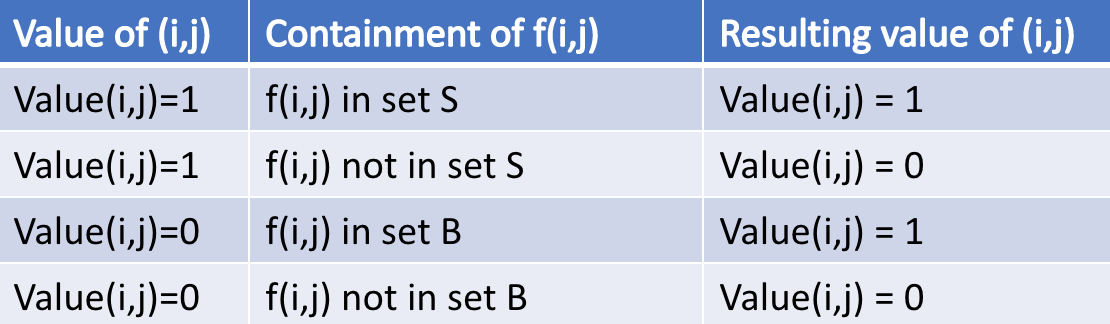
\includegraphics[width=1\linewidth]{EvolutionTable.png}\\

All lattice sites are evolved simultaneously, and a game progresses by continuing to apply these rules to some initial condition.  We can label a game with the terminology of $B \#_1\#_2.../S\#_a\#_b...$, where $B = \{\#_1,\#_2,...\}, S = \{\#_a, \#_b...\}$. In this notation, the Game of Life is $B3/S23$. 

}

\headerbox{Statistical Measures}{name=measures,column=0,below=definitions}{
\textbf{Alive Cell Ratio} Measuring the change in this over the evolution of the system gives a measure of whether a set of rules leads to homogeneity(all alive or all dead), or whether it reaches another equillibrium. \\
\textbf{Displacement from Origin} The mean displacement from the center of the lattice of all alive cells will give a measure of the symmetry of the system. This will be important when we attempt to implement bias. \\
\textbf{Speed} The speed at which a configuration moves away from the origin(defined to be the maximal displacement divided by its evolution time) will be very important when discussing the divergence of configurations and of rule sets more generally.  \\

}

\headerbox{References}{name=references,column=0,below=measures}{
\smaller													% Make the whole text smaller
\vspace{-0.4em} 										% Save some space at the beginning
\bibliographystyle{plain}							% Use plain style
\renewcommand{\section}[2]{\vskip 0.05em}		% Omit "References" title
\begin{thebibliography}{1}							% Simple bibliography with widest label of 1
\itemsep=-0.01em										% Save space between the separation
\setlength{\baselineskip}{0.4em}					% Save space with longer lines
\bibitem{prevWork1} Github: https://github.com/mhaas10/workspace.git
\bibitem{prevWork2} Poster template made by Brian Amberg.
\end{thebibliography}
}


\headerbox{Neighbor Weight Biasing}{name=neighbor,span=1,column=1,row=0}{
A key aspect of the Game of Life is that it has equal neighbor weights, such that $w_0 = w_1 =  \dots = w_7 =1$. This means that the evolution of a configuration has no special preference for any direction, meaning that symmetric configurations will remain symmetric. If we allow variation of these weights, we see that we can implement various types of bias on the evolution of our system.\\

We can use a symmetric initial configuration and the rule set $B34S23$ to demonstrate this bias. For equal weights on the left and an increase in weighting of the upper left corner on the right, we have the following evolutions.

\centering
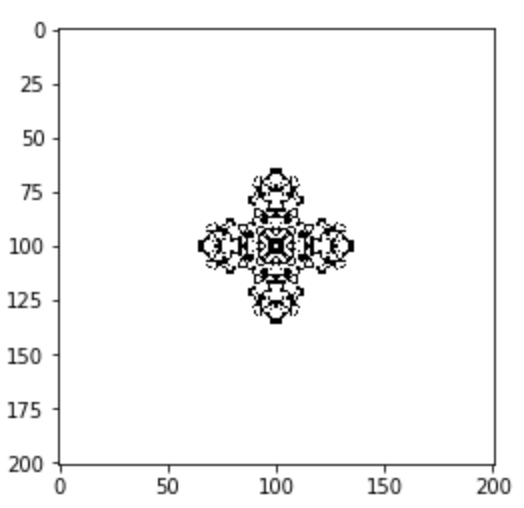
\includegraphics[width=0.4\linewidth]{SymmetricFinal}   vs.
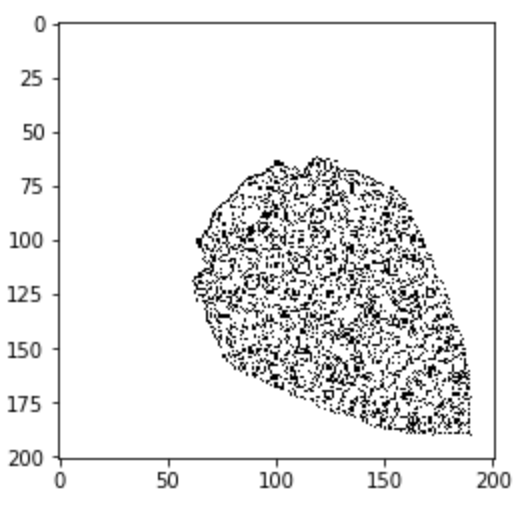
\includegraphics[width=0.4\linewidth]{AsymmetricFinal}


While it is clear from the above that the speed and mean distance has varied as a result of this bias, if we look at the cell ratio graph for these two simulations, we also see that the asymmetric generation rate is more than 4 times as large. 

\centering
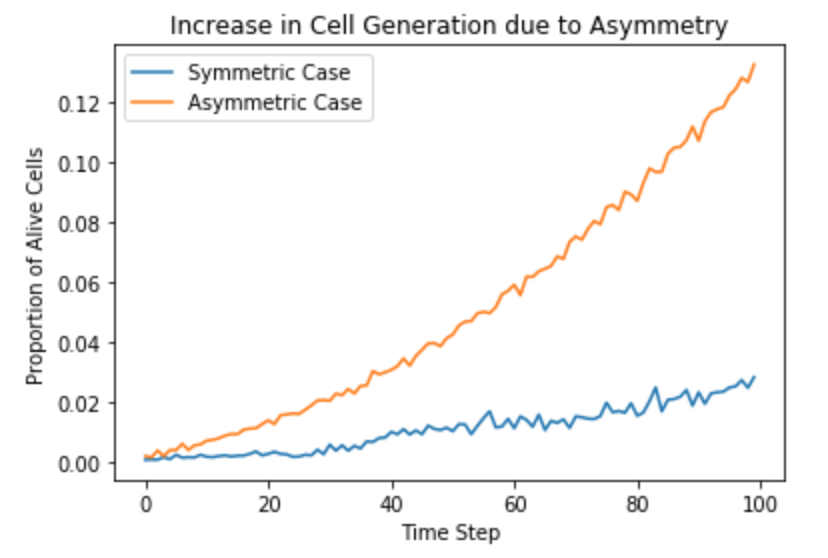
\includegraphics[width=0.6\linewidth]{AliveCountChart}





}
\headerbox{Boundary Conditions}{name=boundary,span=1,column=2,row=0}{
	Another aspect of the Game of Life is that it is played on a periodic boundary. This allows for moving features, like gliders, and expanding features to increase without bound. One interesting alternative to this is to create a boundary that confines the features to a lattice of fixed size.
	
		\centering
	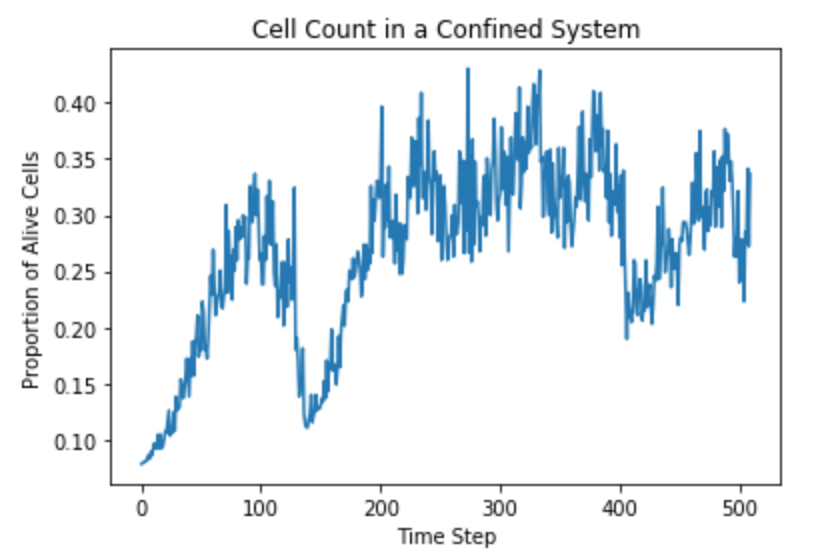
\includegraphics[width=0.4\linewidth]{ConfinedCount}
	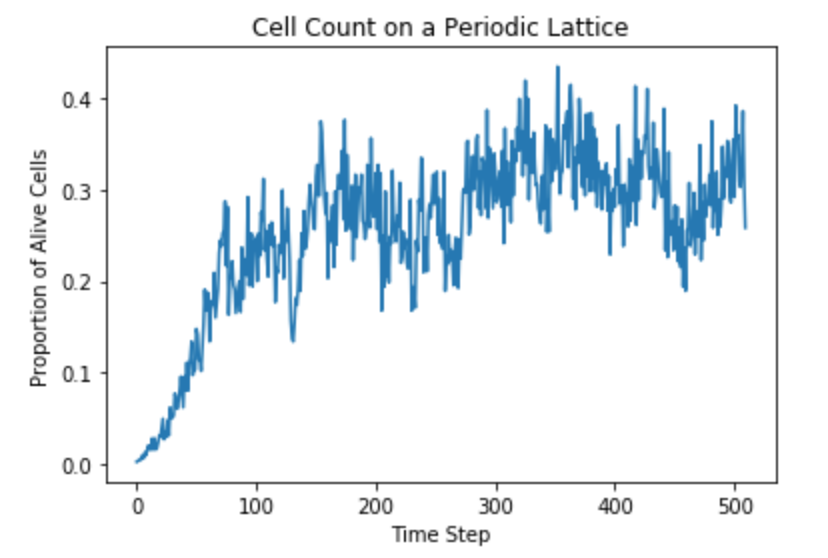
\includegraphics[width=0.4\linewidth]{UnconfinedCount}
	
	
	Once again, we are able to use the alive cell ratio to see that there are some periods of time in which there is destructive interference in the confined lattice that doesn't exist in the periodic lattice case. We can see these by looking at a snapshot within the time period of deconstructive interference. \\
	
	\centering
	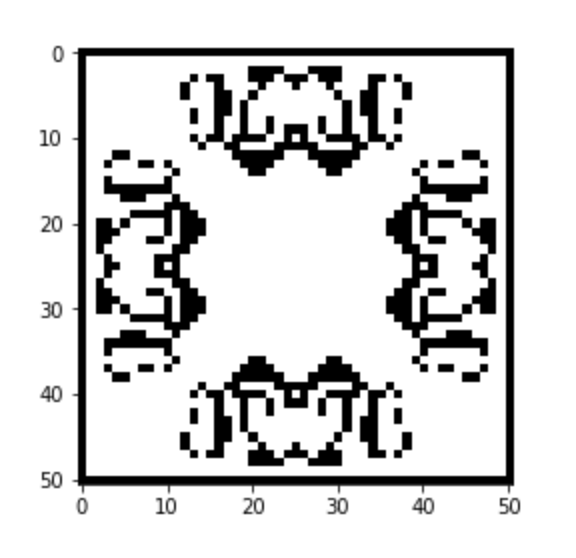
\includegraphics[width=0.4\linewidth]{ConfinedSnapshot}
	
	This result is interesting because the Game of Life has been shown to serve as an excellent generator for emergent properties of physical systems. By seeing that the implementation of boundary walls within a cellular automaton leads to new dynamics, we have the potential to observe the emergence of behavior that exists in waveguides, particles in a box, and other more complex potential landscapes.

	
	
	
	
	
}

\headerbox{Varying over the Rule Sets}
{name=ruleset,span=2,column=1,below=neighbor}{
So far, we have fixed our rule set as $B34S23$ in order to best isolate the features that we have been trying to demonstrate. However, there are 2*8! possible rule sets, which provides for the majority of the variation within the parameter space that we are looking at. We can learn about the behavior of variations in rule sets by comparing the model results of a collection of similar rule sets, $\{BnS25\}$, where $Bn = \{1,2,\dots, n\}$, and we shall let $n\in \{1,3,5,6,7\}$ so we can get a full spectrum. 

\centering
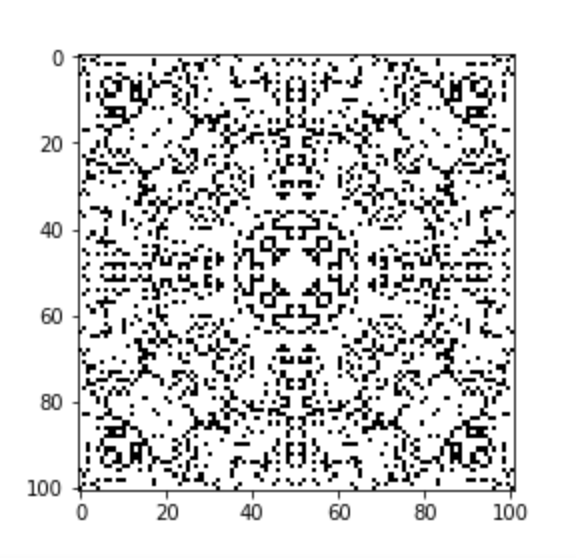
\includegraphics[width=0.19\linewidth]{11} 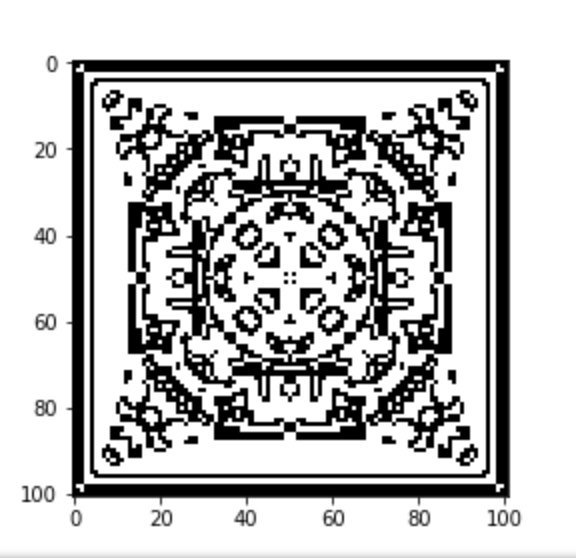
\includegraphics[width=0.19\linewidth]{31}
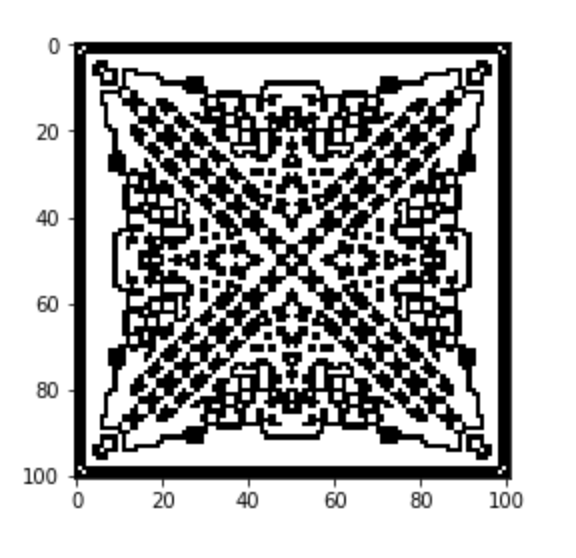
\includegraphics[width=0.19\linewidth]{51}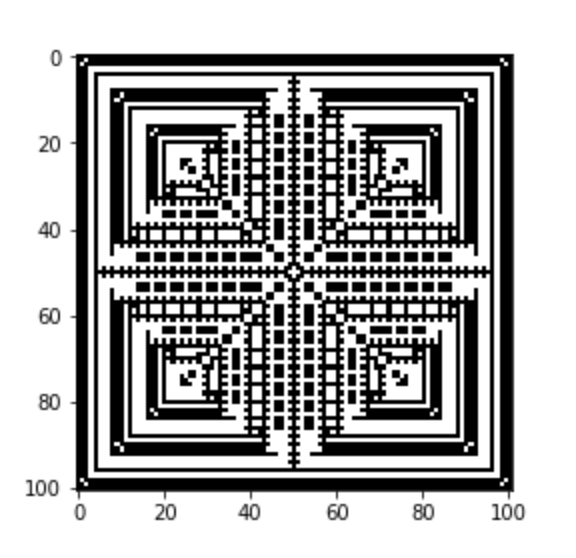
\includegraphics[width=0.19\linewidth]{61}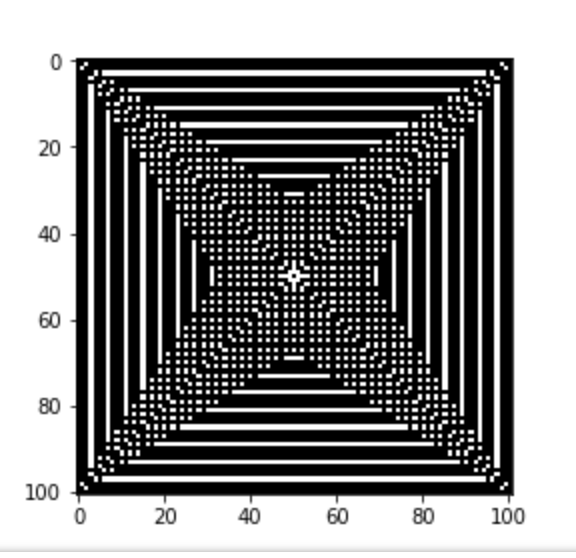
\includegraphics[width=0.19\linewidth]{81}

We see that as we increase the number of $B$ terms, we increase the complexity of the pattern that emerge. This will play a crucial role in how we should interperet shifts in rule sets, since having too few rule set terms will lead to a model with no interesting clusters, whereas saturating a model with too many terms will lead to a highly structured, rigid result. This gives some clarity as to why the Game of Life takes the form it does, in which it has enough terms to lead to interesting dynamics without having so many that the result is constrained by having too many alive cells.
}


\headerbox{Conclusions}
{name=conclusion,span=2,column=1,below=ruleset,above=bottom}{
	We have demonstrated that there are interesting features of the parameter space that are absent from the Game of Life. Knowing that the Game of Life is able to simulate the emergent behavior of some physical systems, we are now able to simulate the behavior of more complex systems. Even more interestingly, if we think of the $B$ terms as terms that promote the "flipping" of a cell, and the $S$ terms as those that inhibit such flipping, we can begin to associate rule sets with some index $T$, which can be thought of in the same way as temperature was in the Ising model, such that a higher index leads to increased flipping of elements. Learning from the Ising model, it would be interesting to see if there is some concept of a phase transition in these systems, and whether this phase transition is related to the temperature for which $B3S23$ is associated. Creating such an association, we would be able to easily find all rule sets that accomplish the balancing act we discussed in the previous section. This would be very interesting to study in the future.
}

\end{poster}
\end{document}
